\section{Orthogonaliteitscompressie}
\label{sec:orthogonaliteitscompressie}

Men zou kunnen denken dat bij de Tuckerdecompositie de meeste ruimte ingenomen wordt door de kerntensor. Wanneer men namelijk naar tensoren met $k$ modes kijkt, waarbij de lengte per mode $n$ constant blijft en telkens gecomprimeerd wordt naar rang $r$, dan groeit de gecomprimeerde kerntensor met $O(r^k)$ en de factormatrices slechts met $O(knr)$, dus met $n, r$ constant en groeiende $k$ worden de factormatrices verwaarloosbaar.\\

In de praktijk werken we echter met een beperkt aantal modes en vaak lage compressierangen. Zelfs als we later reshapen verhogen we hiermee $k$, maar verlagen we $n$ en $r$, dus het aandeel van de kerntensor zal hierdoor niet zozeer veel verhogen. Bijvoorbeeld, wanneer men de ST-HOSVD (met optimizaties) toepast op Cuprite met relatieve doelfout 0.025, comprimeert men van rang (512, 614, 190) naar (139, 192, 4) en nemen de factormatrices 64\% van het geheugen in. Bij Mauna Kea, een veel grotere dataset, is dit percentage 55\%. We kunnen dus concluderen dat het zeker interessant is om te kijken naar specifieke compressietechnieken voor de factormatrices.\\

We weten dat de factormatrices orthogonaal zijn en dit kunnen we benutten. Een factormatrix $U \in \mathbb{R}^{n \times r}$ met $r \leq n$ heeft namelijk $nr$ elementen maar deze zijn onderhevig aan $r(r - 1)/2$ impliciete orthogonaliteitsconstraints (daarnaast zijn er ook $r$ normalisatieconstraints maar deze zijn niet-lineair en zullen we niet behandelen). Het zou dus erg nuttig zijn om per factormatrix $r(r - 1)/2$ elementen minder op te slaan. Om terug te komen op de eerdere voorbeelden: dit zou bij Cuprite en Mauna Kea neerkomen op 9.4\% en 7.5\% van alle waarden (inclusief kerntensor) respectievelijk. In deze sectie bespreken we twee technieken om de factormatrices op te slaan met een beperkt aantal waarden.

\subsection{Methode met stelsels}
\label{subsec:methode-met-stelsels}

Stel, we hebben een factormatrix $U \in \mathbb{R}^{n \times r}$ en verdelen deze op de volgende wijze:
\[
U = \begin{bmatrix}
A & c & \dots \\
B & x & \dots \\
\end{bmatrix}
\]
met $A \in \mathbb{R}^{(n-k) \times k}$, $B \in \mathbb{R}^{k \times k}$, $c \in \mathbb{R}^{n-k}$, $x \in \mathbb{R}^{k}$, voor willekeurige $1 \leq k < n$. Vanwege orthogonaliteit weten we dat:
\begin{align*}
\begin{bmatrix}
A \\
B \\
\end{bmatrix}^T
\begin{bmatrix}
c \\
x \\
\end{bmatrix}
&= 0 \\
A^T c + B^T x &= 0 \\
B^T x &= -A^T c
\end{align*}
Bijgevolg kunnen we $x$ berekenen als de oplossing van een lineair stelsel met $k$ onafhankelijke vergelijkingen en $k$ variabelen en moeten deze waarden niet opgeslagen worden. Theoretisch gezien kan men dus, door dit proces sequentieel uit te voeren voor $k = 1, \dots, n - 1$, een hele driehoek van $r (r - 1)/2$ elementen uit de matrix laten vallen (zie figuur \ref{fig:orthogonality_compression_visual_standard} voor een visualisatie). Men kan ook kiezen om de kolommen in een andere volgorde te verwerken, maar de originele volgorde leek ons het beste zodat de herberekende waarden vooral zitten in de latere singuliere vectoren, die minder belangrijk zijn.\\

\begin{figure}[]
  \centering
  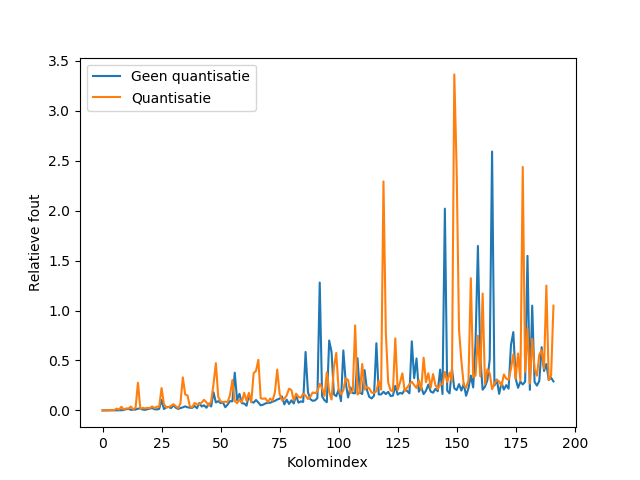
\includegraphics[scale=0.7]{images/orthogonality_compression_basic.png}
  \caption{Relatieve fout van de gereconstrueerde kolommen van de tweede factormatrix van Cuprite met relatieve doelfout 0.025. De relatieve fout van een gereconstrueerde kolom $q_i'$ ten opzichte van de originele kolom $q_i$ is gedefinieerd als $\frac{||q_i' - q_i||}{||q_i||} = ||q_i' - q_i||$ (want $||q_i|| = 1$).}
\label{fig:orthogonality-compression-basic}
\end{figure}

\begin{figure}[]
  \centering
  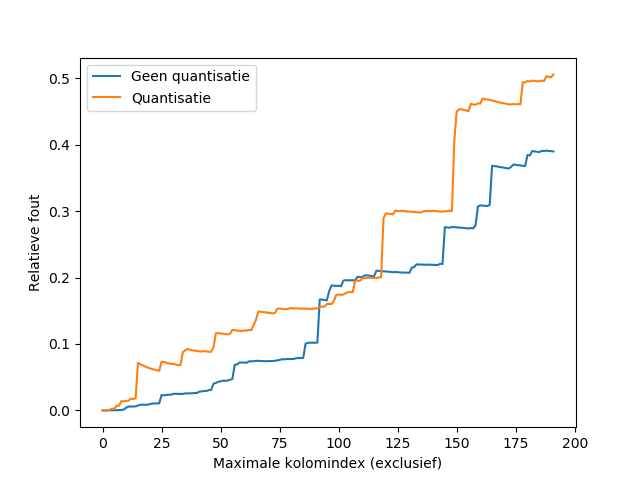
\includegraphics[scale=0.7]{images/orthogonality_compression_basic_matrix.png}
  \caption{Relatieve fout van de eerste kolommen (tot aan de maximale kolomindex, exclusief) van de tweede factormatrix van Cuprite met relatieve doelfout 0.025.}
\label{fig:orthogonality-compression-basic-matrix}
\end{figure}

\begin{figure}[]
\centering
\begin{subfigure}{0.22\textwidth}
  \centering
  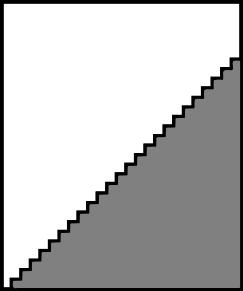
\includegraphics[width=0.9\linewidth]{images/orthogonality_compression1.png}
  \caption{Standaard}
  \label{fig:orthogonality_compression_visual_standard}
\end{subfigure}%
\begin{subfigure}{.22\textwidth}
  \centering
  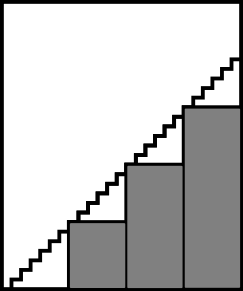
\includegraphics[width=0.9\linewidth]{images/orthogonality_compression2.png}
  \caption{Met 3 blokken}
  \label{fig:orthogonality_compression_visual_blocks}
\end{subfigure}
\begin{subfigure}{.22\textwidth}
  \centering
  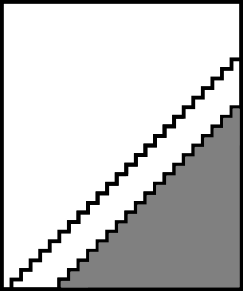
\includegraphics[width=0.9\linewidth]{images/orthogonality_compression3.png}
  \caption{Met marge 5}
  \label{fig:orthogonality_compression_visual_margin}
\end{subfigure}
\begin{subfigure}{.22\textwidth}
  \centering
  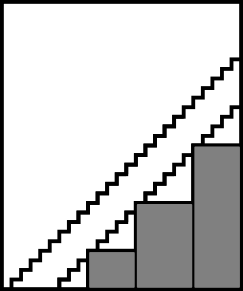
\includegraphics[width=0.9\linewidth]{images/orthogonality_compression4.png}
  \caption{Met beide}
  \label{fig:orthogonality_compression_visual_blocks_margin}
\end{subfigure}
\caption{Een visuele voorstelling van de standaardtechniek en mogelijke aanpassingen. De grijze waarden worden niet opgeslagen.}
\label{fig:orthogonality_compression_visual}
\end{figure}

In de praktijk ligt het echter anders. Om rekening te houden met de quantisatiefase die hierna nog zal behandeld worden, hebben we ook getest wat het effect is van te quantiseren naar 16-bit integers (door de waarden te verschuiven en schalen naar het volledige bereik van dit datatype). In figuren \ref{fig:orthogonality-compression-basic} en \ref{fig:orthogonality-compression-basic-matrix} zien we dat er zowel zonder als met quantisatie significante fouten gemaakt worden in de reconstructie. Sommige vectoren worden gereconstrueerd met extreme waarden en als men goed kijkt naar figuur \ref{fig:orthogonality-compression-basic}, ziet men dat de fout per vector ook stijgt naarmate dat men verder in de matrix is. We blijven namelijk de oplossingen van vorige problemen hergebruiken en hierdoor accumuleren de fouten zich. Als we uiteindelijk deze factormatrices gebruiken voor de decompressie, bekomen we bij Cuprite een relatieve fout op het eindresultaat van 0.0885 zonder en 0.0773 met quantisatie (de doelfout is 0.025).\\

Ten tweede is de uitvoeringstijd van deze methode niet ideaal: de gecombineerde compressie- en decompressietijd voor deze fase is gemiddeld slechts 0.8s voor Cuprite, maar 61.9s bij Pavia Centre, een dataset met grotere factormatrices (in beide gevallen werken we met een relatieve doelfout van 0.025). In de rest van deze subsectie zullen we technieken bespreken in een poging om de fout en rekentijd te beperken. Om zaken ordelijk te houden zullen we ons in deze bespreking beperken tot het geval met quantisatie, aangezien dit ons realistischer lijkt.

\subsubsection{Hernormalisatie}

We zagen eerder dat, aangenomen dat elk stelsel van volle rang is, er wiskundig gezien een unieke oplossing is voor elke gereconstrueerde waarde. In theorie zou deze dan exact moeten overeenkomen met de originele waarde, waardoor alle kolommen vanzelf genormaliseerd zijn. Het enige wat ons algoritme echter expliciet doet is de waarden kiezen zodat de geproduceerde vectoren zo orthogonaal mogelijk staan op de vorige. In figuren \ref{fig:orthogonality-compression-norms1} en \ref{fig:orthogonality-compression-norms2} ziet men de normen van de gereconstrueerde kolommen. Analoog aan de fout, zijn er opnieuw uitschieters en de andere kolommen worden ook steeds minder genormaliseerd naarmate de fouten accumuleren.\\

\begin{figure}[]
  \centering
  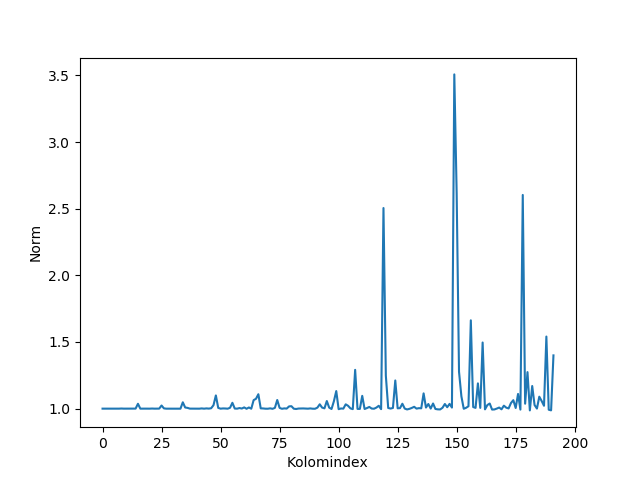
\includegraphics[scale=0.7]{images/orthogonality_compression_norms1.png}
  \caption{Norm van de gereconstrueerde kolommen van de tweede factormatrix van Cuprite met relatieve doelfout 0.025.}
\label{fig:orthogonality-compression-norms1}
\end{figure}

\begin{figure}[]
  \centering
  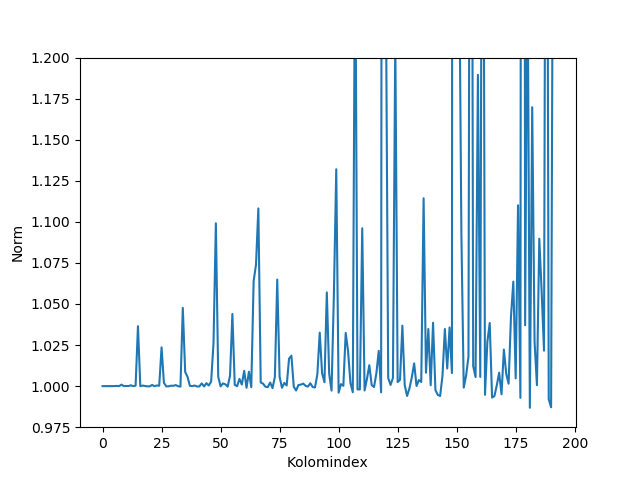
\includegraphics[scale=0.7]{images/orthogonality_compression_norms2.png}
  \caption{Norm van de gereconstrueerde kolommen van de tweede factormatrix van Cuprite met relatieve doelfout 0.025. Naast de uitschieters zijn de latere vectoren ook steeds minder genormaliseerd.}
\label{fig:orthogonality-compression-norms2}
\end{figure}

Een mogelijke oplossing hiervoor is elke kolom na reconstructie expliciet hernormaliseren, inclusief de originele waarden, zodat de richting van de vector niet verandert maar de norm wel altijd klopt. Men ziet in figuur \ref{fig:orthogonality-compression-renormalization} dat de reconstructie al veel beter verloopt. De relatieve fout op het eindresultaat is nu dan ook nog maar 0.0349. Vanwege deze grote verbetering en de kleine kost in rekenwerk zullen we voortaan altijd hernormalisatie gebruiken.

\begin{figure}[]
  \centering
  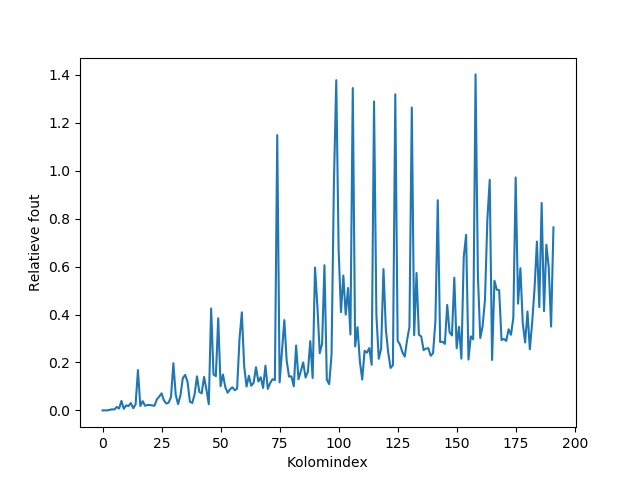
\includegraphics[scale=0.7]{images/orthogonality_compression_renormalization.png}
  \caption{Relatieve fout van de gereconstrueerde kolommen van de tweede factormatrix van Cuprite met relatieve doelfout 0.025 (met hernormalisatie).}
\label{fig:orthogonality-compression-renormalization}
\end{figure}

\begin{figure}[]
  \centering
  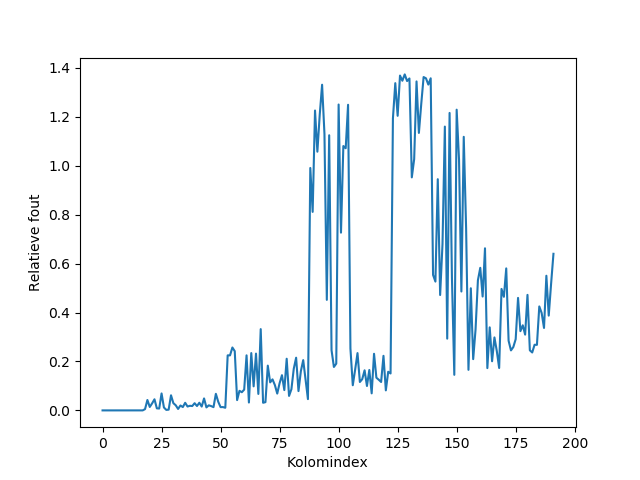
\includegraphics[scale=0.7]{images/orthogonality_compression_blocks.png}
  \caption{Relatieve fout van de gereconstrueerde kolommen van de tweede factormatrix van Cuprite met relatieve doelfout 0.025 (met hernormalisatie en 10 blokken).}
\label{fig:orthogonality-compression-blocks}
\end{figure}

\subsubsection{Blokken}

Een tweede aanpassing die men kan maken is om te werken met blokken van kolommen in plaats van individuele kolommen. Enerzijds verbetert dit misschien de fout, omdat de ketting van het hergebruiken van uitvoer als invoer korter wordt, maar dit geeft vooral een grote verbetering in rekentijd. Voor een co\"effici\"entenmatrix met afmetingen $k \times k$ kost het oplossen van $b$ onafhankelijke stelsels namelijk $O(bk^3)$ tijd. Echter, wanneer deze stelsels dezelfde matrix delen en alleen verschillen in de rechterhandzijde, kan men \'e\'en keer de LU-factorizatie van de matrix berekenen en dan snel elk stelsel oplossen, wat leidt tot een complexiteit van $O(k^3 + bk^2)$. Het nadeel hiervan is dat we wel meer waarden moeten opslaan (zie figuur \ref{fig:orthogonality_compression_visual_blocks}), waardoor de compressiefactor verlaagt.\\

We voerden een experiment uit met 10 blokken. In figuur \ref{fig:orthogonality-compression-blocks} ziet men dat voor Cuprite de fout helaas niet daalt, sterker nog: de uiteindelijke relatieve fout is nu 0.0357. Men kan zien dat veel kolommen beter gereconstrueerd worden maar sommige blokken hebben een slechte co\"effici\"entenmatrix waardoor er een grote fout komt op de volledige blok. Aan de andere kant daalt de rekentijd enorm, zoals verwacht, tot een gemiddelde van 0.06s voor Cuprite en 1.48s voor Pavia Centre. In tabel \ref{table:orthogonality-compression-systems-summary} op het einde van deze subsectie ziet men trouwens dat de fout voor Pavia Centre wel verbetert. Dit hangt dus van geval tot geval af.

\begin{figure}[H]
  \centering
  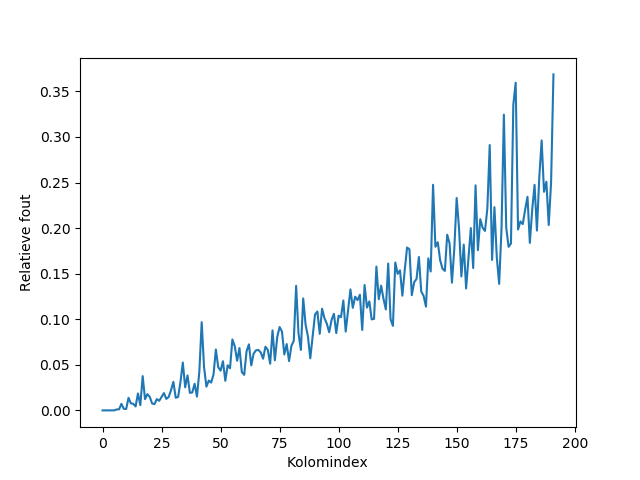
\includegraphics[scale=0.7]{images/orthogonality_compression_margin.png}
  \caption{Relatieve fout van de gereconstrueerde kolommen van de tweede factormatrix van Cuprite met relatieve doelfout 0.025 (met hernormalisatie en marge 3).}
\label{fig:orthogonality-compression-margin}
\end{figure}

\newpage
\subsubsection{Marge}

Ten derde kan men de compressiefout afwegen tegen de compressiefactor door een extra marge op te slaan per kolom (zie figuur \ref{fig:orthogonality_compression_visual_margin}). Hierdoor wordt het stelsel overgedetermineerd en zullen we eigenlijk \textit{least-squares}-problemen oplossen. Met deze toegevoegde informatie kunnen we hopelijk een accuratere oplossing berekenen. Figuur \ref{fig:orthogonality-compression-margin} toont ons dat dit ook in de praktijk werkt: met marge 3 is de relatieve fout op het eindresultaat gedaald tot 0.0257.

\subsubsection{Hergebruik vorige stelsels}

Onze huidige methode lost een reeks stelsels of least-squares-problemen op die telkens een deel van de co\"effici\"entenmatrix delen met het vorige probleem, zonder dat we hier gebruik van maken. Voor een vierkante matrix met constante blokgrootte en marge resulteert dit in een complexiteit van $O(n^4)$, wat erg hoog is. We vermoeden dat men, door eerder rekenwerk te hergebruiken, dit algoritme kan optimaliseren en misschien zelfs de complexiteit kan reduceren tot $O(n^3)$. We zullen dit echter niet verder analyseren vanwege de goede resultaten van de methode met Householder-reflecties (zie de volgende subsectie).

\subsubsection{Samenvatting}

In tabel \ref{table:orthogonality-compression-systems-summary} ziet men een samenvattende vergelijking tussen de technieken besproken in deze subsectie. De gemiddelde uitvoeringstijden voor Pavia Centre zijn nog niet volledig geconvergeerd bij deze steekproefgrootte, maar men kan wel duidelijke trends zien. Qua compressiefactoren zijn er geen grote verschillen: hernormalisatie heeft hier geen invloed op, een marge van 3 weinig en door te werken met 10 blokken worden slechts ongeveer 9\% van de waarden die anders weggefilterd werden, bijgehouden. Als men deze methode gebruikt kan men het aantal blokken of de grootte van de marge beschouwen als parameters, die eventueel geoptimaliseerd kunnen worden.

\begin{table}[H]
\centering
\begin{tabular}{|l|c|c|c|c|}
\hline
\multirow{2}{*}{} & \multicolumn{2}{c|}{Relatieve fout} & \multicolumn{2}{c|}{Totale tijd (s)} \\ \cline{2-5} 
 & Cuprite & Pavia Centre & Cuprite & Pavia Centre \\ \hline
\input{data/orthogonality-compression-systems-summary.tex}                             
\end{tabular}
\caption{Vergelijking tussen de standaard methode met stelsels en verschillende aanpassingen (10 experimenten). Totale tijd wijst hier op zowel compressie- als decompressietijd voor deze fase (geen ST-HOSVD).}
\label{table:orthogonality-compression-systems-summary}
\end{table}

\newpage
\subsection{Methode met Householder-reflecties}

Er bestaat een alternatieve methode om orthogonale matrices compact op te slaan, namelijk gebaseerd op het algoritme voor het berekenen van de QR-factorizatie met Householder-reflecties \cite{ref:qr_factorization_householder}. Hierbij worden niet de waarden van de matrix zelf opgeslagen, maar getransformeerde waarden die met extra operaties redelijk precies de originele matrix kunnen reconstrueren.\\

De QR-factorizatie van een matrix $U$ schrijft de matrix uit als een product van een orthogonale matrix $Q$ met een bovendriehoeksmatrix $R$. Een van de manieren om deze factorizatie op een numeriek stabiele manier te berekenen is aan de hand van Householder-reflecties. Dit zijn lineaire transformaties van de vorm:
\[
H = I - 2vv^T
\]
Elke reflectie wordt dus gedefinieerd door een vector $v$. Men kan voor een arbitraire vector $x$ een $v$ berekenen zodat $Hx = (\alpha, 0, \dots, 0)^T$, met $\alpha$ een scalar. In de eerste iteratie van het algoritme kiest men dan $v_1$ zodat de eerste kolom van $U$ gereflecteerd wordt op \'e\'en as. Daarna past men een reflectie toe op de matrix $H_1 U$ zonder de eerste rij en kolom (dus de eerste rij en kolom van $H_2$ zijn gelijk aan die van de eenheidsmatrix en de rest van de matrix is een Householder-reflectiematrix gebaseerd op een vector $v_2$ van \'e\'en dimensie lager). Dit proces blijft men toepassen voor elke kolom, totdat men de bovendriehoeksmatrix $R = H_r H_{r-1} \dots H_1 U$ bekomt. De orthogonale matrix $Q$ is dan gelijk aan $H_1^{-1} H_2^{-1} \dots H_r^{-1}$.\\

We zien dus dat men de $Q$ van een QR-factorizatie compacter kan opslaan aan de hand van de reflectoren. Onze orthogonale matrices $U_i$ zijn echter afkomstig uit een SVD dus we kennen deze reflectoren niet. We lossen dit op door simpelweg een QR-factorizatie uit te voeren op onze matrices. Namelijk, als $U$ al orthogonaal is, dan zal $R$ gelijk zijn aan de eenheidsmatrix op de tekens na (deze worden door het algoritme gekozen), dus alleen de tekens moeten opgeslagen worden. $Q$ daarentegen kan voorgesteld worden door vectoren $v_1, \dots, v_r$ van dimensie $n, \dots, n - r + 1$. Deze reflectoren passen juist in de onderdriehoek van de originele matrix dus met deze methode zouden we exact de compressie moeten kunnen bereiken die we zoeken.\\

Zoals bij de methode met stelsels zouden we de kolomvolgorde kunnen aanpassen, maar de originele volgorde lijkt ons opnieuw goed; de eerste kolom wordt namelijk alleen bepaald door de eerste reflectie, terwijl de laatste kolom bepaald wordt door alle reflecties. De eerste kolommen zullen dus met hogere precisie herberekend worden, wat ons goed uitkomt (zie ook subsectie \ref{sec:quantisatie-factor-matrices}).\\

Verder zijn de verwijderde elementen niet willekeurig gekozen, maar bijna gelijk aan -1, 0 of 1 op afrondingsfouten na (de elementen van $R$). Tijdens de procedure wordt de norm per kolom ook bewaard door de reflecties waardoor men geen last heeft van \textit{catastrophic cancellation} zoals bij de Gram-Schmidt-procedure. Deze methode zou dus numeriek stabieler moeten zijn dan de methode met stelsels.\\

Helaas bieden de meeste libraries QR-factorizatie alleen aan in zijn volledige vorm, waarbij de eerste stap (het opstellen van de reflectors) en de tweede stap (het berekenen van $Q$ zelf) niet gescheiden kunnen worden door de gebruiker. We zouden dit algoritme ook zelf kunnen implementeren in Python, maar de \textit{interpreter} zou voor een grote vertraging zorgen. Gelukkig hebben we via \texttt{scipy.linalg.lapack} toegang tot de nodige LAPACK-routines: \texttt{sgeqrf} (eerste stap) en \texttt{sorgqr} (tweede stap).\\

LAPACK gebruikt een licht gewijzigde notatie voor de reflecties:
\[
H_i = I - \tau_i v_i v_i^T
\]
waarbij $v_i$ niet genormalizeerd is maar $\sqrt{\frac{\tau_i}{2}} v_i$ wel en $\tau_i$ zo gekozen wordt dat $(v_i)_1 = 1$, zodat het nog steeds gaat om een Householder-reflectie maar LAPACK de diagonaalposities in de originele matrix niet nodig heeft om het eerste element van de reflectors bij te houden. In plaats hiervan geeft men als uitvoer zowel de originele matrix (waarin $R$ in de bovendriehoek en de reflectoren in de overige posities opgeslagen worden) als een vector $\tau$ van dimensie $r$.\\

Zoals eerder gezegd hebben we nog de tekens van $R$ nodig om $U$ te reconstrueren. Op zich zou \'e\'en bit per kolom opslaan weinig moeite kosten, maar het leek ons toch ordelijker om dit te doen in de uitvoer die we al hebben. We weten namelijk dat elke waarde $\tau_i$ gelijk is aan 0 als er in iterate $i$ geen reflectie nodig was, of anders $1 \leq \tau_i \leq 2$ \cite{ref:slarfg}. We kunnen dus de $r$ tekens van $R$ opslaan in de tekens van $\tau$, waarbij eventuele nul-elementen vervangen worden door een waarde die duidelijk verschilt van 0, zoals 0.5.

\begin{table}[H]
\centering
\footnotesize
\begin{tabular}{|l|c|c|c|c|}
\hline
\multirow{2}{*}{} & \multicolumn{2}{c|}{Relatieve fout} & \multicolumn{2}{c|}{Totale tijd (s)} \\ \cline{2-5} 
 & Cuprite & Pavia Centre & Cuprite & Pavia Centre \\ \hline
\input{data/orthogonality-compression-householder-summary.tex}                             
\end{tabular}
\normalsize
\caption{Experimentele resultaten van de methode met Householder-reflecties. De eerste rij is een referentie zonder orthogonaliteitscompressie (dus een pure ST-HOSVD) en de derde rij quantiseert zoals beschreven in subsectie \ref{subsec:methode-met-stelsels} (10 experimenten). Totale tijd wijst hier op zowel compressie- als decompressietijd voor deze fase (orthogonaliteitscompressie en eventuele quantisatie, geen ST-HOSVD).}
\label{table:orthogonality-compression-householder-summary}
\end{table}

In tabel \ref{table:orthogonality-compression-householder-summary} staan de experimentele resultaten van de methode met Householder-reflecties. We zien dat de rekentijd enorm verbeterd is vergeleken met de methode met stelsels. Dit algoritme vraagt dan ook maar $O(n^3)$ rekenwerk en wordt bijna volledig ge\"implementeerd in LAPACK. Daarnaast is de ge\"introduceerde fout verwaarloosbaar voor onze toepassing.\\

Aangezien deze methode zo precies is kijken we best ook eens naar het effect van grovere quantisatie dan 16-bit. Figuur \ref{fig:orthogonality-compression-householder-quantisation-bits} toont de evolutie van de fout in functie van het aantal quantisatiebits bij Cuprite. Men ziet dat voor een laag aantal bits er zeker een significante fout is. Een manier om deze methode nog een beetje te verbeteren is hernormalisatie: we schalen elke vector $v_i$ (op het eerste element na, dat sowieso 1 is maar niet wordt opgeslagen) met een factor zodat $\sqrt{\frac{\tau_i}{2}} v_i$ genormaliseerd is.

\begin{figure}[H]
  \centering
  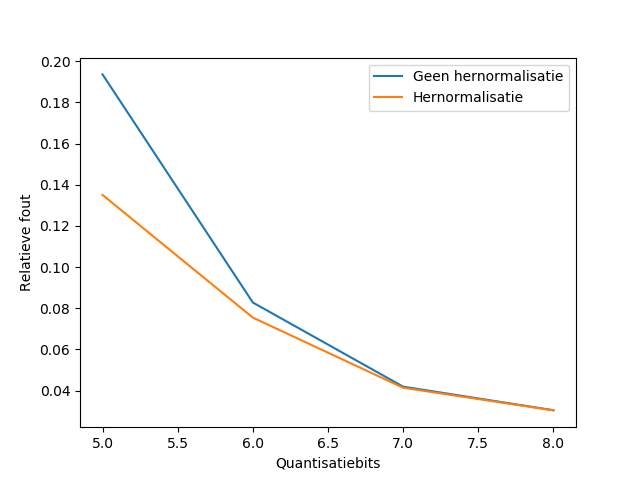
\includegraphics[scale=0.7]{images/orthogonality_compression_householder_quantisation_bits.png}
  \caption{Relatieve fout van het eindresultaat bij Cuprite met relatieve doelfout 0.025 (met en zonder hernormalisatie van de reflectoren).}
\label{fig:orthogonality-compression-householder-quantisation-bits}
\end{figure}

We zien in figuur \ref{fig:orthogonality-compression-householder-quantisation-bits} dat hernormalisatie een merkbare verbetering geeft voor een laag aantal quantisatiebits en zullen deze techniek dus vanaf nu gebruiken, al maakt het weinig uit voor een groter aantal bits, vanwege de kleine hoeveelheid toegevoegd rekenwerk. In onze experimenten hier is $\tau$ weliswaar niet gequantiseerd, maar zoals besproken wordt in sectie \ref{sec:quantisatie} is dit sowieso geen slecht idee aangezien men slechts \'e\'en waarde per kolom per factormatrix moet opslaan en dat deze waarde effect heeft op de volledige reflector.\\

Ten slotte zou men kunnen denken dat het ook nuttig is om de gereconstrueerde factormatrix terug te orthogonaliseren en normaliseren. Echter, eens dat de reflectoren genormaliseerd zijn, zijn de Householder-transformatiematrices orthogonaal en zal het product van deze met de eenheidsmatrix ook orthogonaal zijn. Weliswaar zullen er bij deze transformaties kleine numerieke fouten gemaakt worden, maar deze zijn verwaarloosbaar voor onze toepassing.

\subsection{Besluit}

Aangezien de methode met Householder-reflecties quasi geen fout toevoegt, erg snel werkt en exact $nr - r(r - 1)/2$ waarden moet bijhouden (het theoretische minimum als men alleen kijkt naar de orthogonaliteitsconstraints), verslaat deze duidelijk de methode van de stelsels en zal deze vanaf nu gebruikt worden om de factormatrices compacter op te slaan. Deze methode is ook makkelijker om mee te werken, aangezien er geen parameters afgesteld moeten worden.